\qrchapter{https://forgottenpillar.com/rsc/en-fp-chapter4}{Revision of “Living Temple”}


\qrchapter{https://forgottenpillar.com/rsc/en-fp-chapter4}{Marekebisho ya “Living Temple”}


In \textit{Testimonies for the Church Containing Letters to Physicians and Ministers Instruction to Seventh-Day Adventists}, the tenth chapter, \textit{The Foundation of our Faith,} God gave valuable lessons on the development and consequences of Kellogg's theories. The broader and deeper meaning of these quotations can be understood when we are familiar with their historical context. Let us first take a brief look at the historical context of Kellogg's book, The \textit{Living Temple}.


Katika \textit{Testimonies for the Church containing Letters to Physicians and Ministers Instruction to Seventh-Day Adventist}, sura ya kumi, \textit{Msingi wa Imani yetu,} Mungu alitoa masomo ya thamani kuhusu maendeleo na matokeo ya nadharia za Kellogg. Maana ya kina ya dondoo hizi zinaweza kueleweka tunapofahamu muktadha wao ya kihistoria. Hebu kwanza tuangazie kwa ufupi muktadha wa kihistoria wa kitabu cha Kellogg, The \textit{Living Temple}.


In a series of providence, God signified that “\textit{Living Temple}” should not be printed. One such event was the burning of Battle Creek's press building, just the night before it was to be printed. Finally, the book was printed elsewhere; it instigated a great crisis in the Seventh-day Adventist Church. On October 7, 1903, a annual meeting of the conference was held in Washington DC. Many Seventh-day Adventist church leaders were present, including Dr. Kellogg and his sympathizers. Major controversy was taking place over this book and the conflict was inevitable. Fortunately, on the brink of this escalating conflict, a letter from Sister White was delivered to the council. On Sunday, the letter fell upon the ears of all, to which there resounded many “amen's” and “halleluyah's”. It was a very tense and moving morning for the church that was on the verge of a split—to at last have concrete direction from the Lord's messenger:


Kwa majaliwa, Mungu alionyesha kwamba “\textit{Living Temple}” haipaswi kuchapishwa. Matukio ya ajabu kama vile kuchomwa kwa jengo la waandishi wa habari la Battle Creek, usiku wa kuamkia siku ya kuchapishwa, yalitokea. Hatimaye, kitabu hicho kilichapishwa mahali pengine; kitabu kilizua mgogoro mkubwa katika Kanisa la Waadventista Wasabato. Mnamo Oktoba 7, 1903, mkutano wa kila mwaka wa Conference ulifanyika Washington DC. Viongozi wengi wa kanisa la Waadventista Wasabato walikuwepo, wakiwemo Dk. Kellogg na wafuasi wake. Mabishano makubwa yalikuwa yakifanyika juu ya kitabu hiki na mzozo haukuepukika. Kwa bahati nzuri, wakati mgogoro huu ulichacha sana, barua kutoka kwa Dada White iliwasilishwa kwa baraza. Siku ya Jumapili, barua hiyo ilianguka kwenye masikio ya wote, na kutokana nayo, zilisikika “amina” na “haleluya” nyingi. Ilikuwa asubuhi yenye wasiwasi na yenye kusisimua kwa ajili ya kanisa lililokuwa karibu kugawanyika—hatimaye kuwa na mwelekeo thabiti kutoka kwa Mjumbe wa Bwana:


\begin{figure}[h]
    \centering
    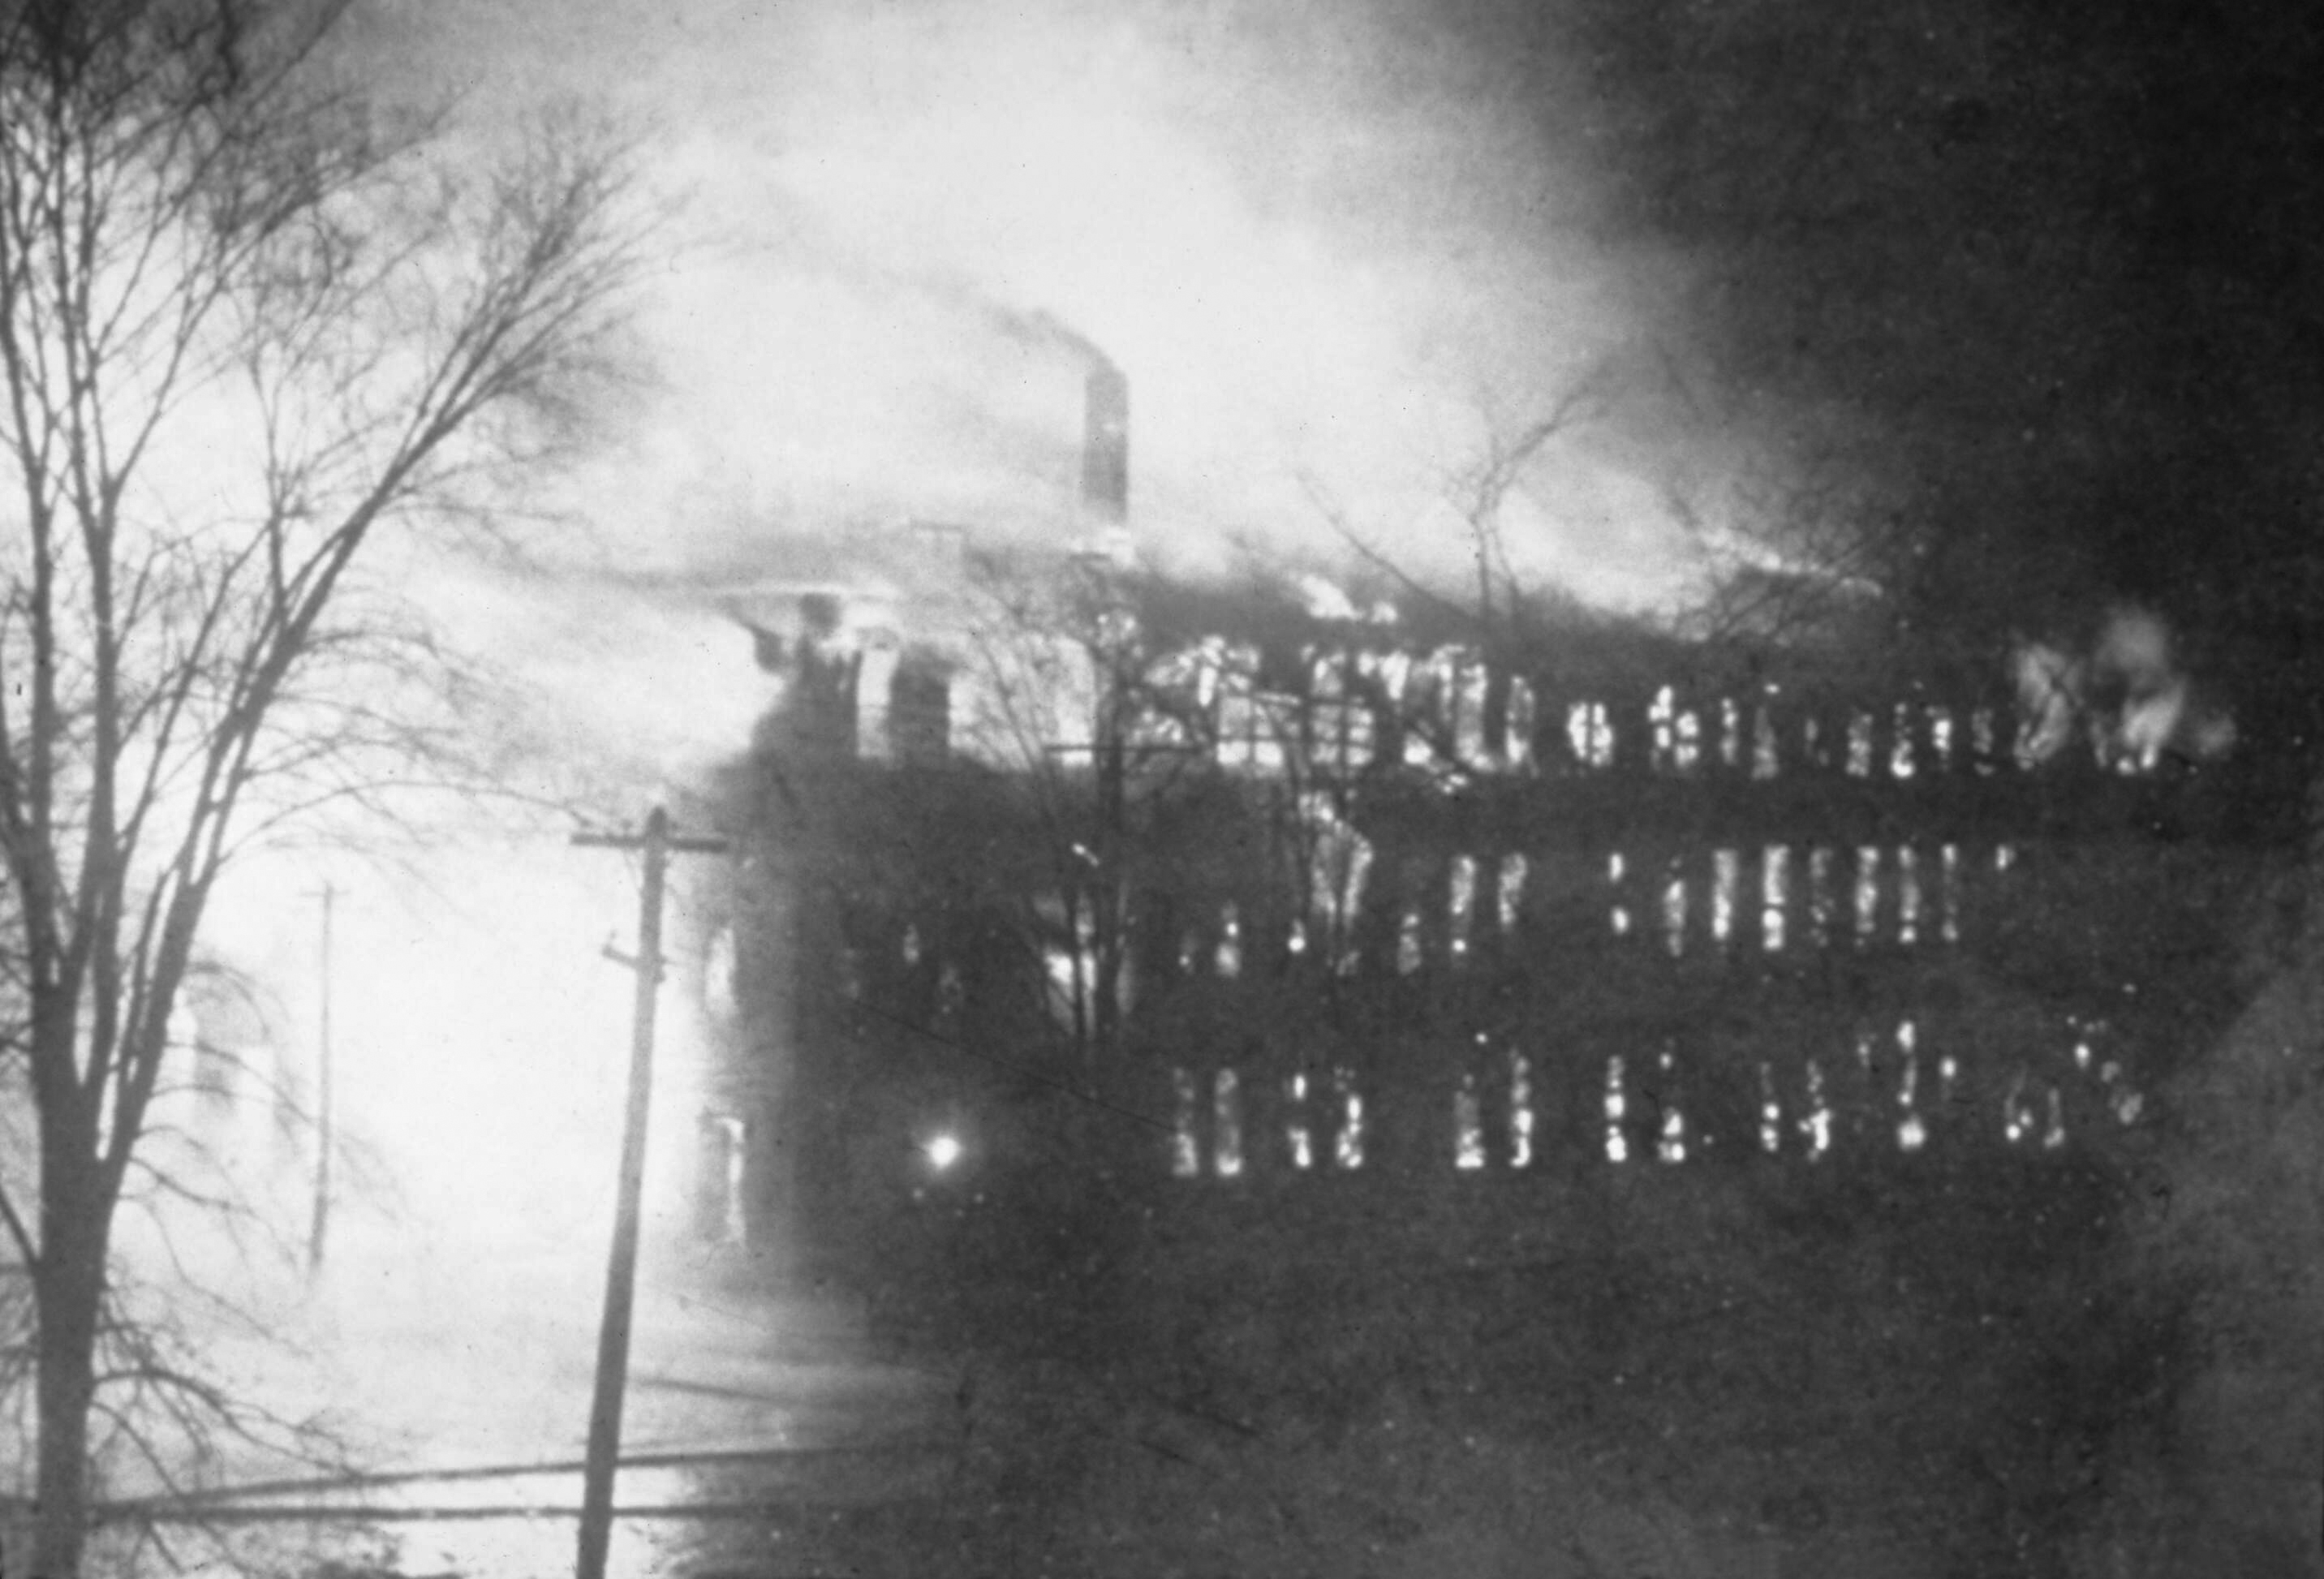
\includegraphics[width=1\linewidth]{images/review-and-herlad.jpg}
    \caption*{Burning of Review and Herald press building, December 30, 1902.}
    \label{fig:review-and-herald}
\end{figure}


\begin{figure}[h]
    \centering
    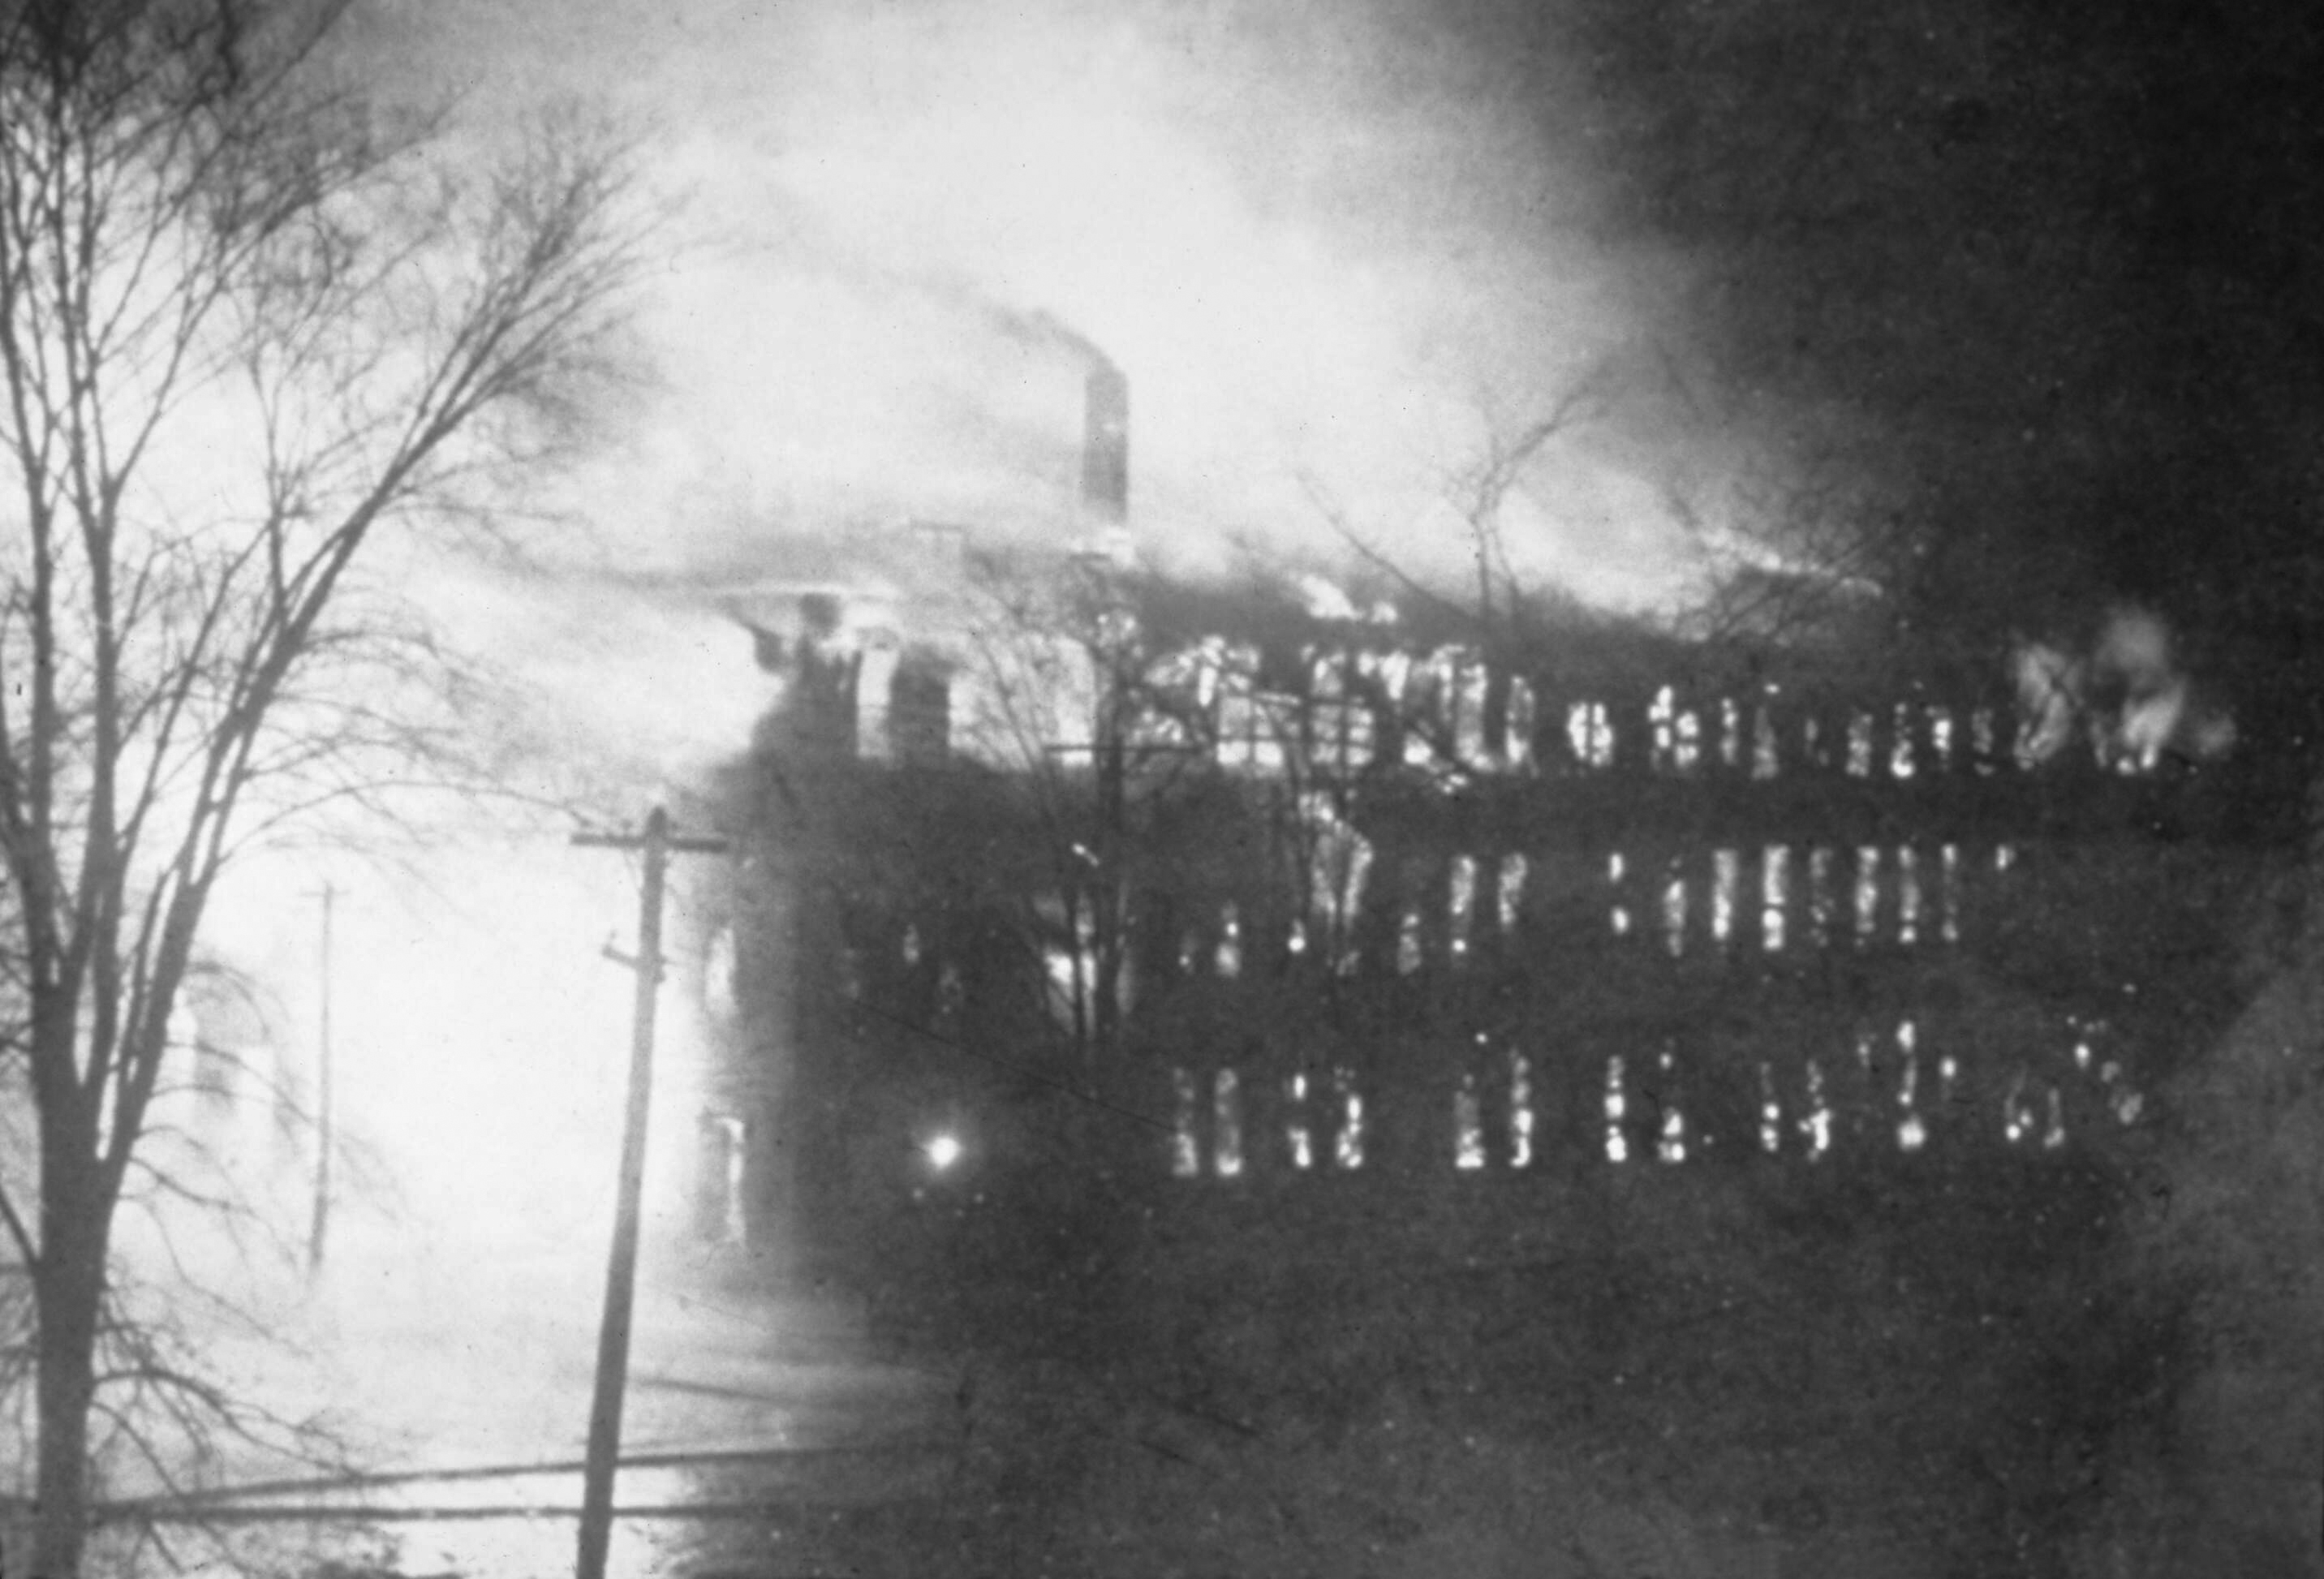
\includegraphics[width=1\linewidth]{images/review-and-herlad.jpg}
    \caption*{Kuchomwa kwa jengo la uchapishaji la Review and Herald, Desemba 30, 1902.}
    \label{fig:review-and-herald}
\end{figure}


\egw{I have some things to say to our teachers in reference to \textbf{the new book The Living Temple}. \textbf{Be careful how you sustain \underline{the sentiments of this book regarding the personality of God}}. As the Lord presents matters to me, \textbf{these sentiments do not bear the endorsement of God}. \textbf{They are a snare that the enemy has prepared for these last days}. I thought that this would surely be discerned and that it would not be necessary for me to say anything about it. \textbf{But since the claim has been made that the teachings of this book can be sustained by statements from my writings, I am compelled to speak in denial of this claim}. There may be in this book expressions and sentiments that are in harmony with my writings. And there may be in my writings many statements which when taken from their connection, and interpreted according to the mind of the writer of Living Temple, would seem to be in harmony with the teachings of this book. \textbf{This may give apparent support to the assertion that the sentiments in Living Temple are in harmony with my writings}. \textbf{But God forbid that this opinion should prevail}.}[Lt211-1903.1; 1903][https://egwwritings.org/read?panels=p14068.9598008]


\egw{Nina mambo fulani ya kuwaambia walimu wetu kuhusiana na \textbf{kitabu kipya The Living Temple}. \textbf{Kuwa mwangalifu kwa ajili ya hoja za kitabu hiki kuhusu \underline{ubinafsi wa Mungu}}. Kulingana na yale ambayo Bwana amewasilisha kwangu, \textbf{hoja hizi hazina uthibitisho wa Mungu}. \textbf{Ni mtego ambao adui ameweka siku hizi za mwisho}. Nilifikiri kwamba hii ingetambuliwa na kwamba haingenilazimu kusema lolote. \textbf{Lakini kwa vile madai yametolewa kuwa mafundisho ya kitabu hiki yanaweza kudumishwa na maandishi yangu, ninalazimika kuongea ili kukana madai haya}. Kunaweza kuwa katika kitabu hiki misemo ambayo inapatana na maandishi yangu. Na kunaweza kuwa katika maandishi yangu kauli nyingi ambazo zikitolewa kwenye miktadha yao, na kufasiriwa kulingana na mawazo ya mwandishi wa Living Temple, zingeonekana kuwa zinapatana na mafundisho ya kitabu hiki. \textbf{Hii inaweza kutoa dhana kuwa hoja za Living Temple zinapatana na maandishi yangu}. \textbf{Lakini Mungu azuie ushindi wa maoni haya}.}[Lt211-1903.1; 1903][https://egwwritings.org/read?panels=p14068.9598008]


Repeatedly, Sister White stated that the true problem of the book was the sentiments\egwinline{\textbf{regarding the personality of God}}. These sentiments are not sustained by statements from Ellen White's writings and these very sentiments\egwinline{\textbf{are a snare that the enemy has prepared for these last days}}.


Mara kwa mara, Dada White alisema kwamba tatizo la kweli la kitabu hicho lilikuwa maoni\egwinline{\textbf{kuhusu ubinafsi wa Mungu}}. Maoni haya haziungwi mkono na kauli kutoka kwa maandishi ya Ellen White na maoni zizi hizi\egwinline{\textbf{ni mtego ambao adui ametayarisha kwa siku hizi za mwisho}}.


God, again in His providence, solved this conflict. Kellogg accepted the reproof from the Lord's messenger and, before the council closed, he stated that the Living Temple would be taken from the market\footnote{\href{https://forgottenpillar.com/wp-content/uploads/2022/04/Letter-A-G-Daniells-to-W-C-White-October-29-1903.pdf}{Letter: A. G. Daniells to W. C. White, October 23, 1903, pp. 5}}. But after the conference, he spoke privately with the general conference president, Brother Arthur G. Daniells, about his plans for revising the book. The following is a look at select letters, revealing Kellogg's plans for revising “\textit{Living Temple}”.


Mungu, tena katika majaliwa yake, alitatua mgogoro huu. Kellogg alikubali karipio kutoka kwa mjumbe wa Bwana na, kabla ya baraza kufungwa, alisema kwamba Living Temple ingetolewa sokoni\footnote{\href{https://forgottenpillar.com/wp-content/uploads/2022/04/Letter-A-G-Daniells-to-W-C-White-October-29-1903.pdf}{Letter: A. G. Daniells to W. C. White, October 23, 1903, pp. 5}}. Lakini baada ya mkutano huo, alizungumza faraghani na rais wa mkutano mkuu, Ndugu Arthur G. Daniells, kuhusu mipango yake ya kurekebisha kitabu hicho. Tutaangazia barua kadhaa zinazofichua mipango ya Kellogg ya kurekebisha “\textit{Living Temple}”.


Ellen White was not present at the yearly conference in Washington DC but her son, William C. White, did attend. When the conference was over, brother Arthur G. Daniells wrote a confidential letter to William C. White regarding Dr. Kellogg's plan to revise his book:


Ellen White hakuwepo katika mkutano wa kila mwaka huko Washington DC lakini mwanawe, William C. White, alihudhuria. Mkutano ulipoisha, ndugu Arthur G. Daniells aliandika barua ya siri kwa William C. White kuhusu mpango wa Dk. Kellogg wa kurekebisha kitabu chake:


\others{October 29, 1903}


\others{Oktoba 29, 1903}


\othersnogap{Ever since the \textbf{council closed} I have felt that I should write you \textbf{confidentially regarding Dr. Kellogg's plans for revising and republishing ‘The Living Temple’}…. He \normaltext{[Kellogg]} said that some days before coming to the council, he had been thinking the matter over, and began to see that \textbf{he had made a slight mistake in expressing his views}. He said that all the way along he had been troubled to know how to state the character of God and his relation to his creation works…}


\othersnogap{Tangu \textbf{baraza lilipofungwa} nimeona nikuandikie \textbf{kwa siri kuhusiana na mipango ya Dk. Kellogg ya kurekebisha na kuchapisha upya ‘The Living Temple’}…. Yeye \normaltext{[Kellogg]} alisema kwamba siku kadhaa kabla ya kufika kwenye baraza, alikuwa akitafakari jambo hilo, na alianza kuona kwamba \textbf{alifanya makosa kidogo katika kutoa maoni yake}. Alisema wakati huo wote wa kucharaza hisia zake ametatizika kujua jinsi ya kutaja tabia ya Mungu na vile vile jinsi Mwenyezi anahusiana na kazi zake za uumbaji...}


\begin{figure}[hp]
    \centering
    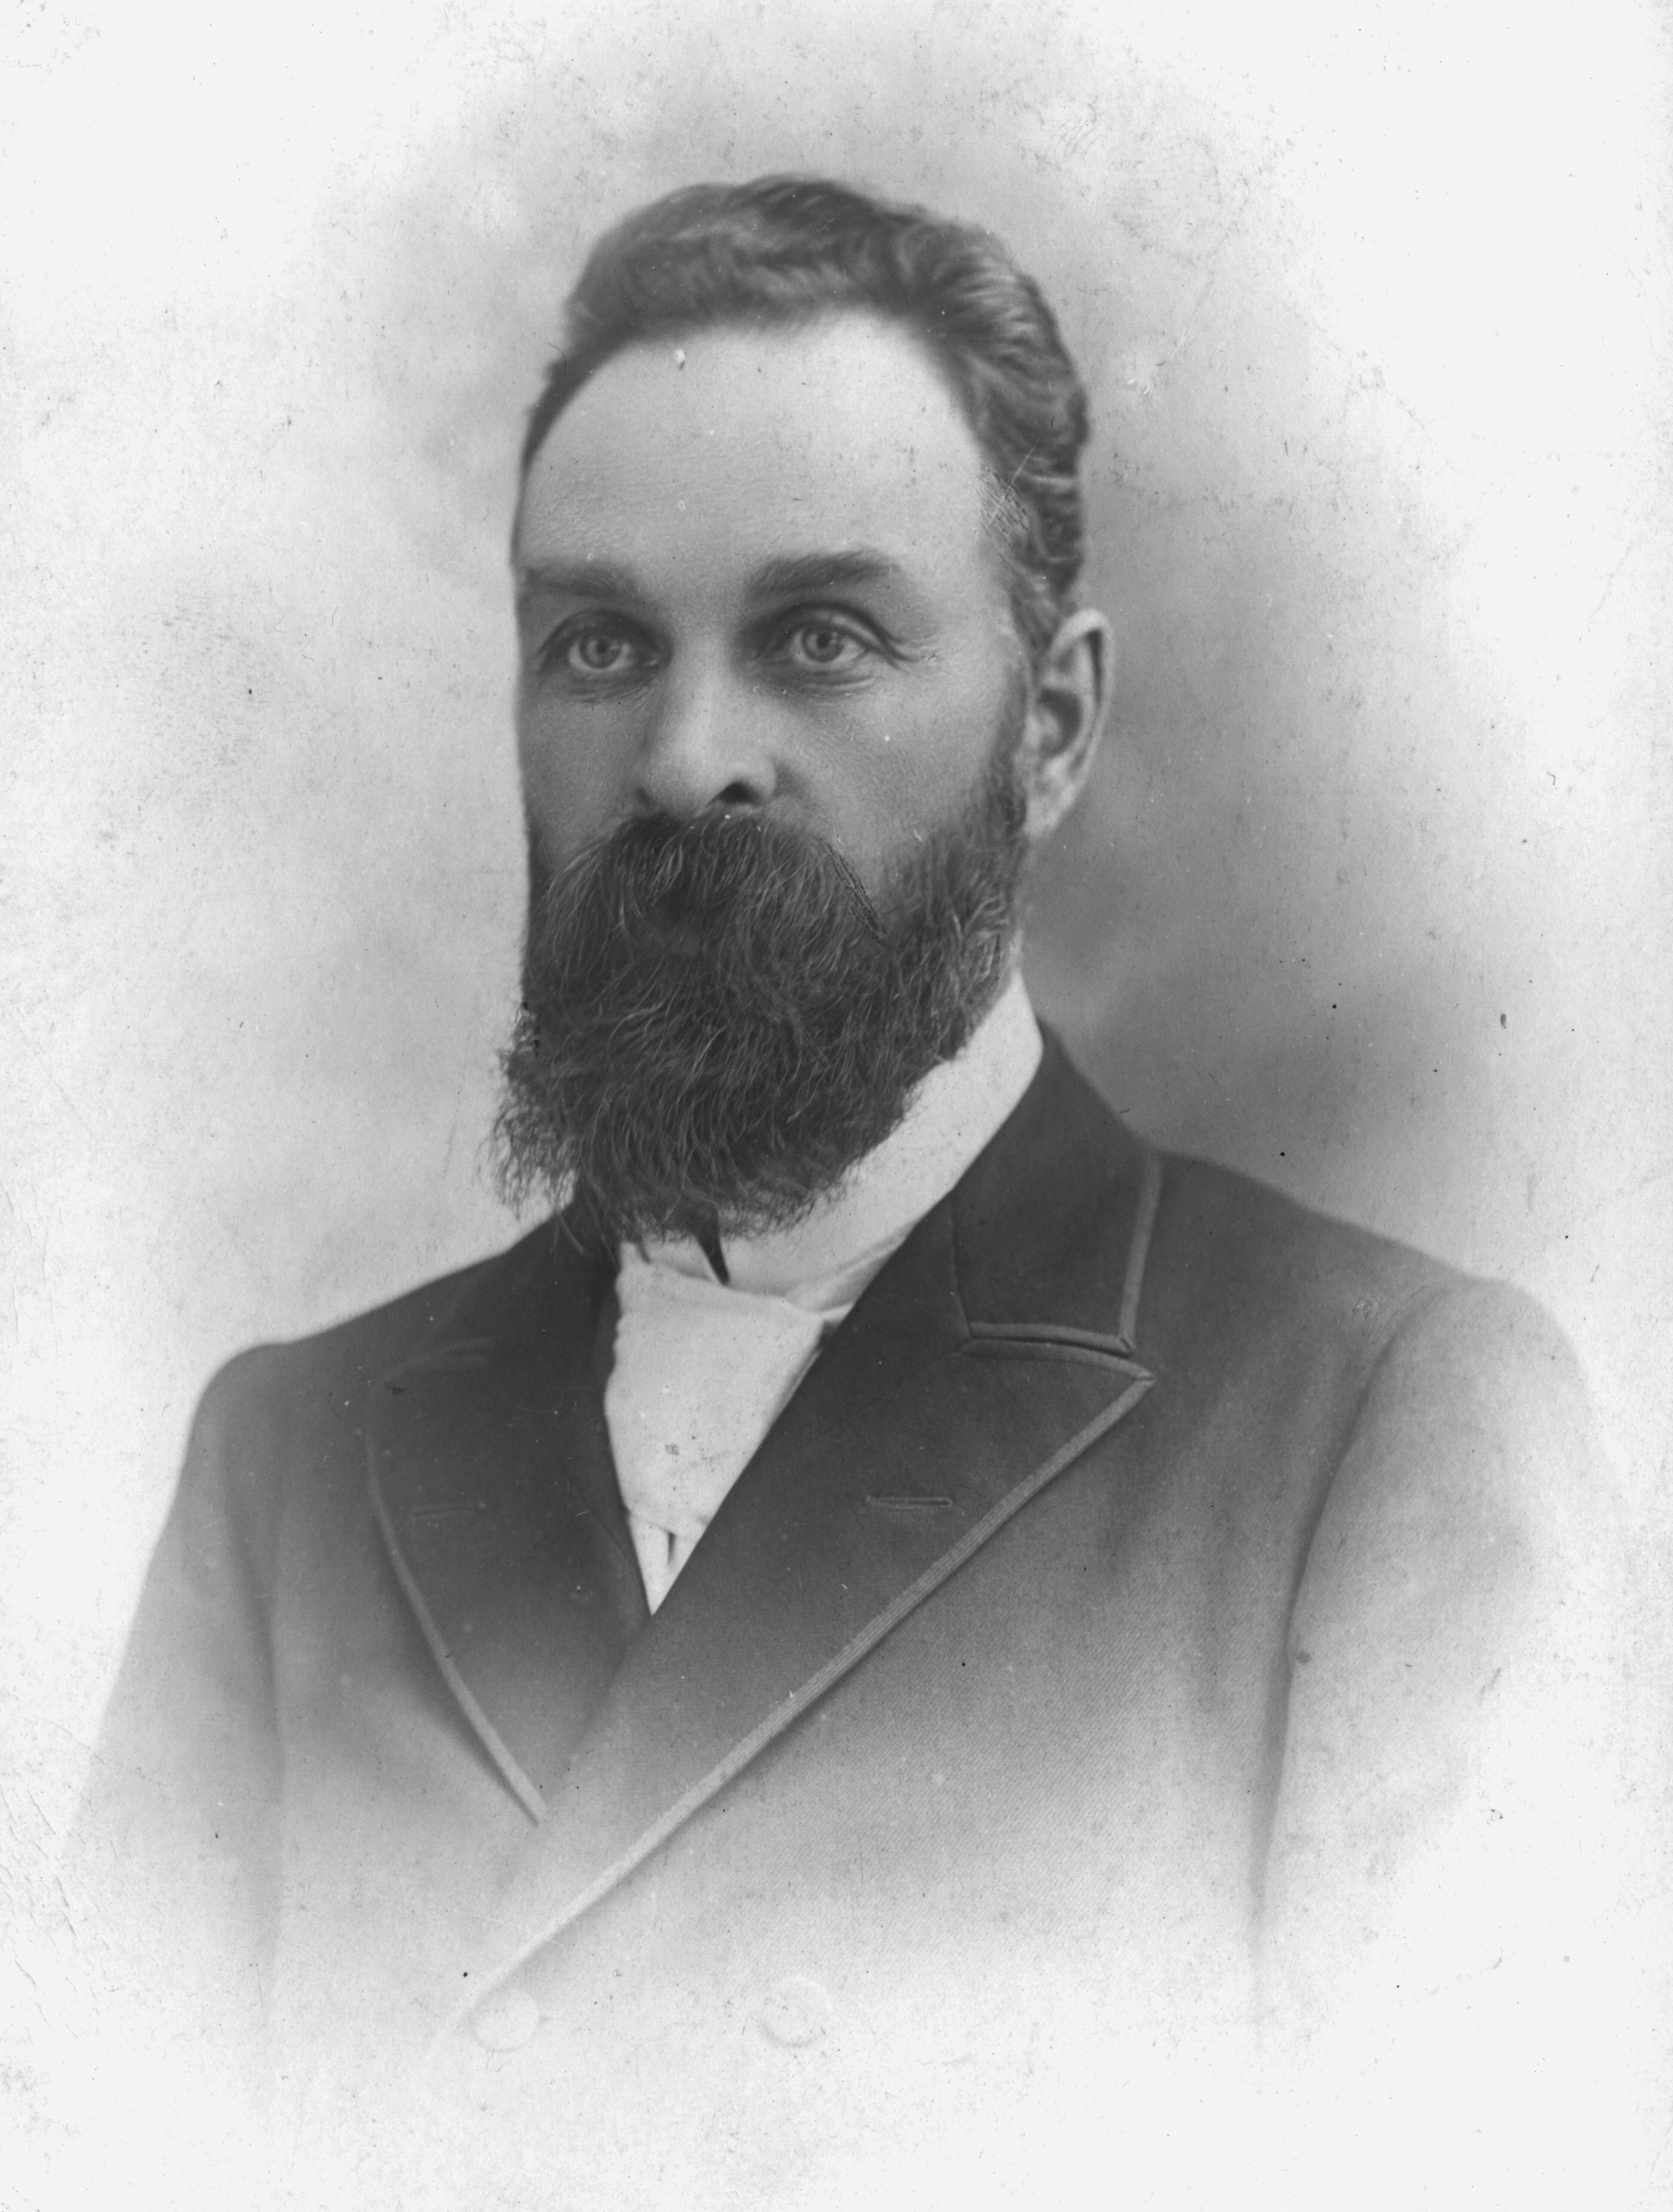
\includegraphics[width=1\linewidth]{images/daniels.jpg}
    \caption*{Arthur Grosvenor Daniells (1858-1935)}
    \label{fig:daniells}
\end{figure}


\begin{figure}[hp]
    \centering
    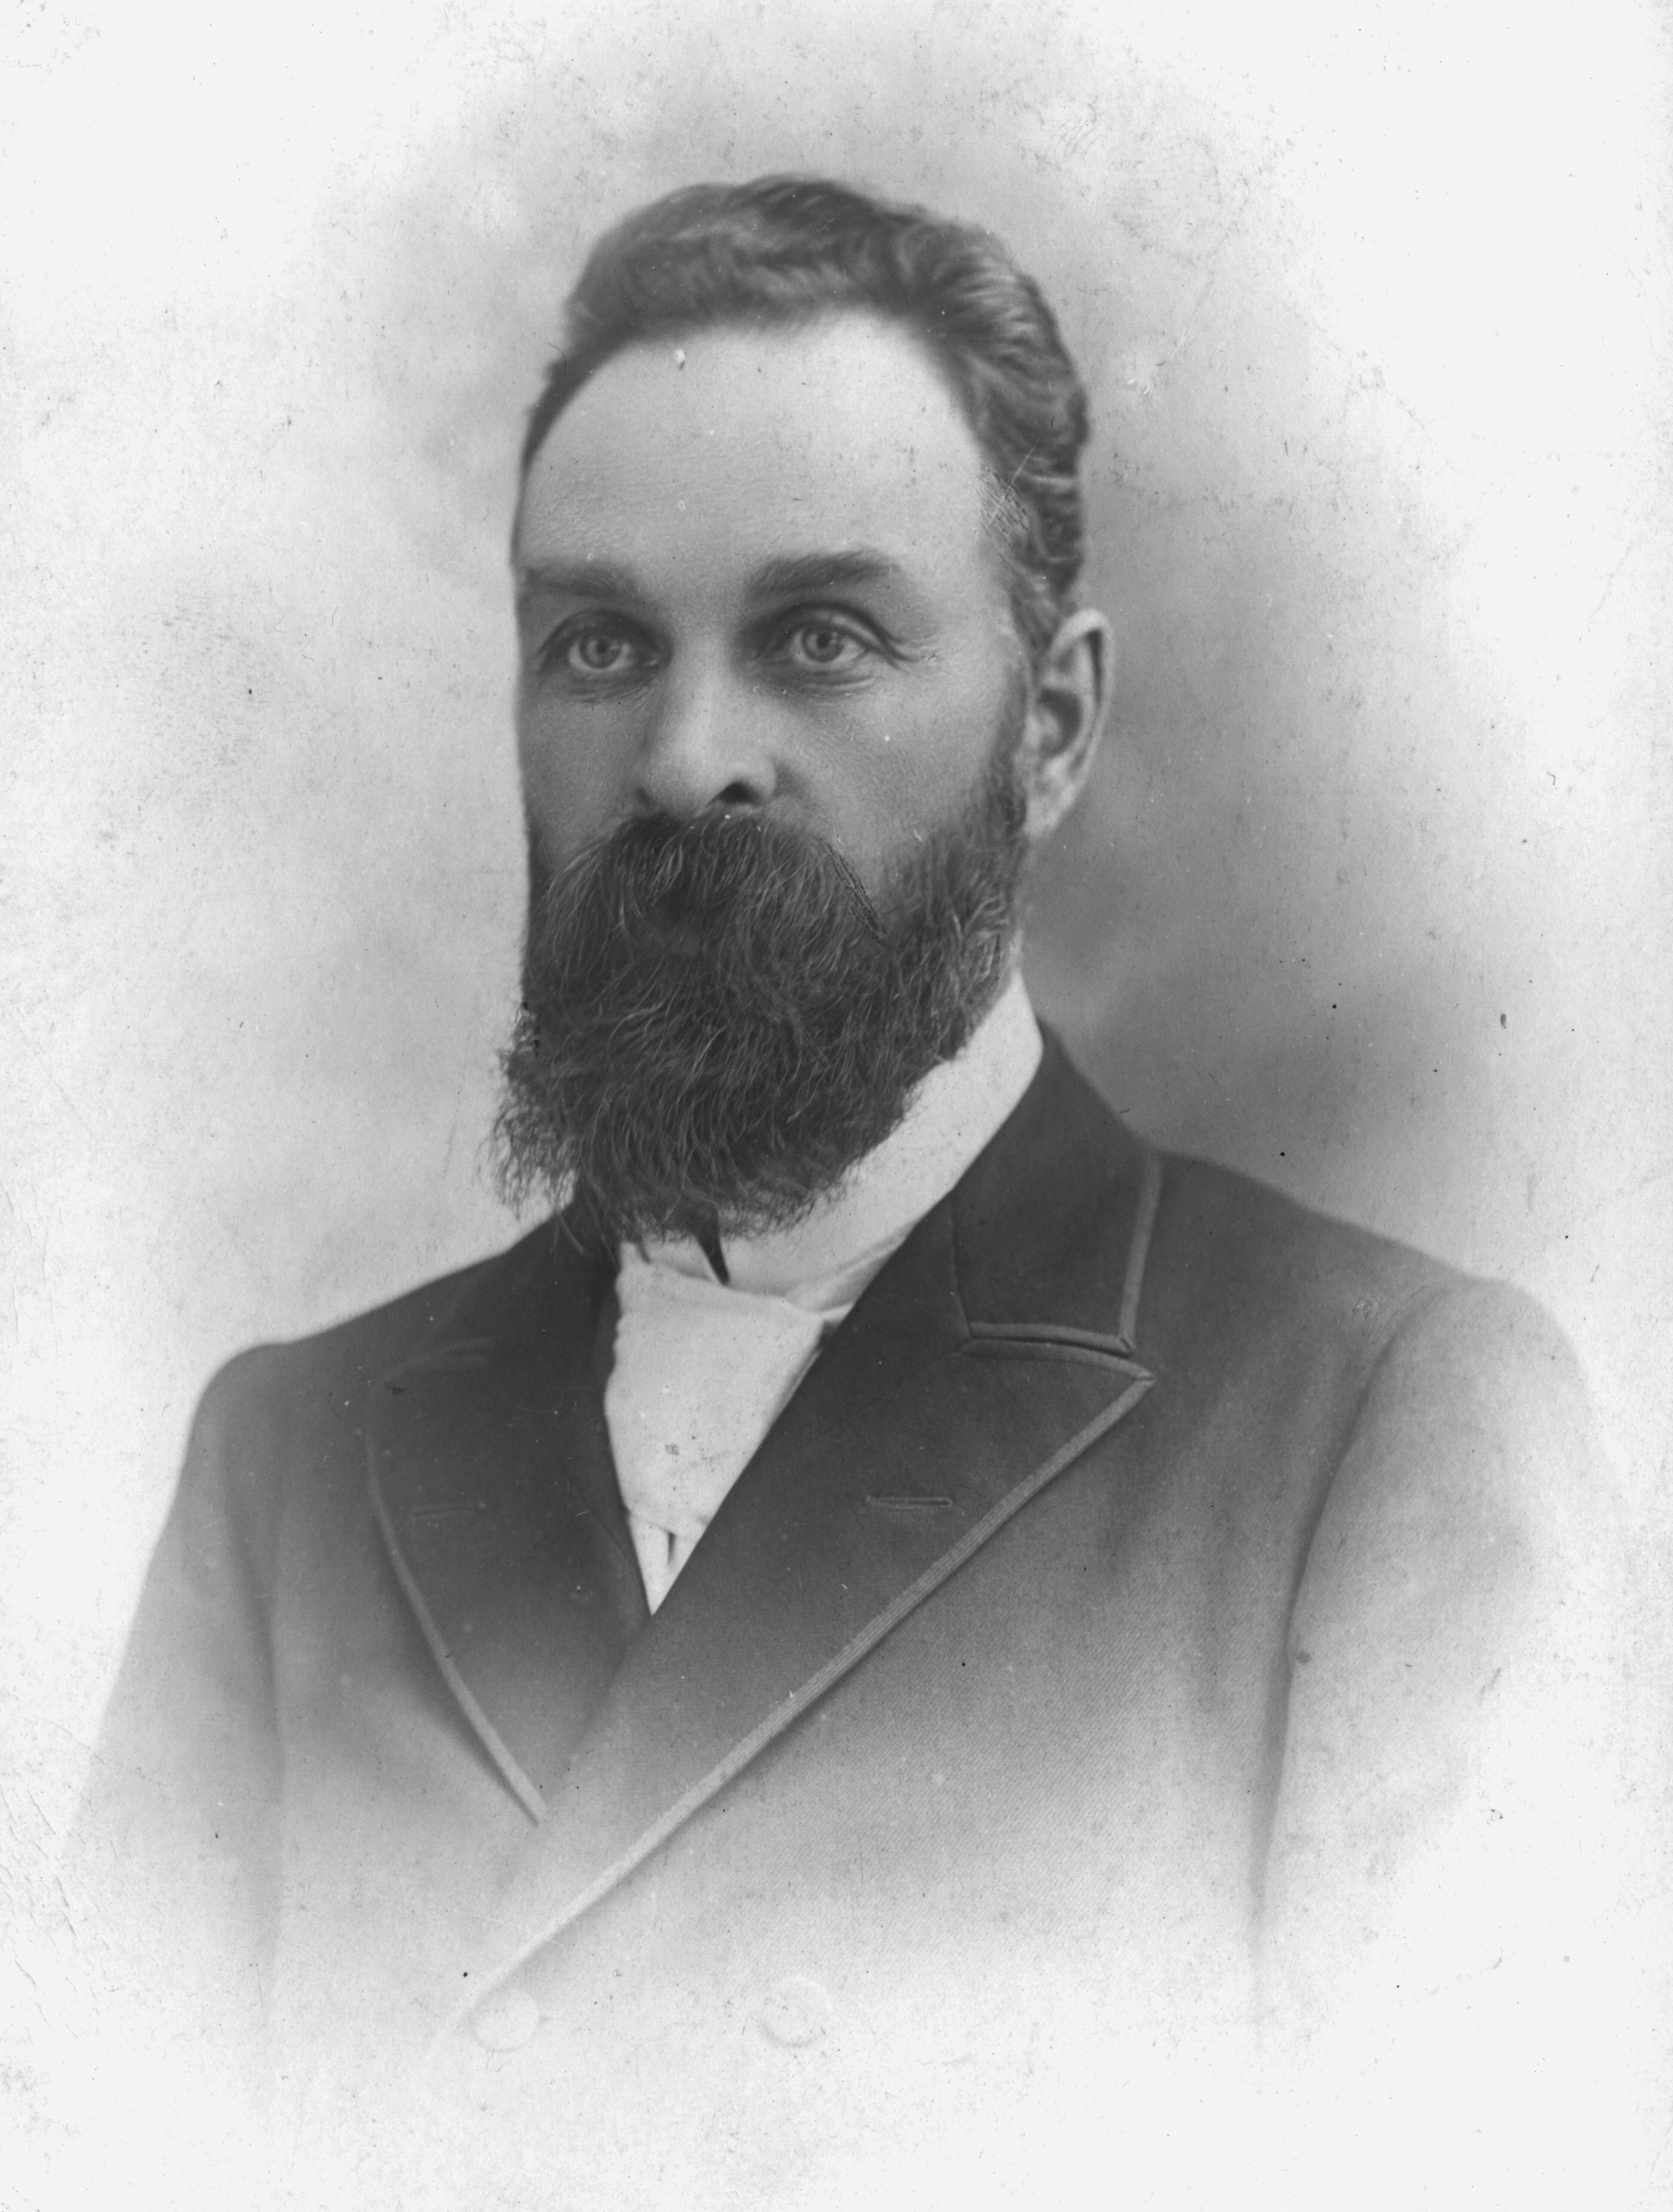
\includegraphics[width=1\linewidth]{images/daniels.jpg}
    \caption*{Arthur Grosvenor Daniells (1858-1935)}
    \label{fig:daniells}
\end{figure}


\othersnogap{\textbf{He then stated that his former views \underline{regarding the trinity} had stood in his way of making a clear and absolutely correct statement; but that within a short time \underline{he had come to believe in the trinity} and could now see pretty clearly where all the difficulty was, and believed that he could clear the matter up satisfactorily.}}


\othersnogap{\textbf{Kisha akasema kwamba maoni yake ya awali \underline{kuhusu utatu} yalikuwa yamemzuia kutoa kauli iliyo wazi na sahihi kabisa; lakini kwa muda mfupi \underline{amekuwa mwaminifu katika fundisho la utatu} na kwa hivyo kwa wakati huu anayo mtazamo toshelezi kung'amua bila tashwishi pale ambapo ugumu wote ulikuwa, na aliamini kwamba angeweza kusuluhisha jambo hilo kwa njia ya kuridhisha.}}


\othersnogap{\textbf{He told me that he now believed in \underline{God the Father, God the Son, and God the Holy Ghost}; and his view was that it was God the Holy Ghost, and not God the Father, that filled all space, and every living thing. He said if he had believed \underline{this} before writing the book, he could have expressed his views without giving the wrong impression the book now gives.}}


\othersnogap{\textbf{Aliniambia kwamba sasa anaamini katika \underline{Mungu Baba, Mungu Mwana, na Mungu Roho Mtakatifu}; na maoni yake yalikuwa kwamba ilikuwa ni Mungu Roho Mtakatifu, na si Mungu Baba, aliyejaza nafasi zote, na kila kiumbe lililohai. Alisema angeliamini \underline{hili} kabla ya kuandika kitabu, angeweza kutoa maoni yake bila kutoa maoni ya-siyofaa jinsi kitabu sasa kinatoa.}}


\othersnogap{\textbf{I placed before him the objections I found in the teaching, and tried to show him that the teaching was so utterly contrary to the gospel that I did not see how it could be revised by changing a few expressions.}}


\othersnogap{\textbf{Niliweka mbele yake pingamizi nilizozipata katika mafundisho hayo, na kujaribu kumwonyesha hiyo mafundisho yalikuwa kinyume kabisa na injili na hivi kwamba sikuona jinsi inavyoweza kurekebishwa kwa kubadilisha misemo michache tu.}}


\othersnogap{We argued the matter at some length in a friendly way; but I felt sure that when we parted, the doctor did not understand himself, nor the character of his teaching. And I could not see how it would be possible for him to flop over, \textbf{and in the course of a few days \underline{fix the books up} so that it would be all right}.}[Letter: A. G. Daniells to W. C. White, October 29, 1903. pp. 1, 2][https://forgotten-pillar.s3.us-east-2.amazonaws.com/Letter-A-G-Daniells-to-W-C-White-October-29-1903.pdf]


\othersnogap{Tulibishana katika suala hilo kwa muda fulani kwa njia ya kirafiki; lakini nilihisi kuwa tulipoachana, daktari hakujielewa mwenyewe, wala kiini cha mafundisho yake. Na sikuweza kuona jinsi gani itakuwa inawezekana kwa yeye \textbf{kubadilisha kikamilifu na kwa wakati wa siku chache \underline{kurekebisha kitabu} ili maoni yaliyowasilishwa yawe sawasawa}.}[Letter: A. G. Daniells to W. C. White, October 29, 1903. pp. 1, 2][https://forgotten-pillar.s3.us-east-2.amazonaws.com/Letter-A-G-Daniells-to-W-C-White-October-29-1903.pdf]


Kellogg did not see the mistake in his sentiments; but rather, in expressing his views. He did not think that his views were false, merely his expression of those views, which led to the book giving a wrong impression. Yet, evidently, this was not true. As Sister White had stated, Kellogg had a problem with the sentiments regarding the \emcap{personality of God} and where His presence is. So, Kellogg suggested that in order to “\textit{fix the books up}” he would include the trinitarian expressions because he now started to believe in \textit{the Trinity} doctrine. At this point in time, the Seventh-day Adventist Church was not trinitarian—the doctrine of Trinity was not part of the \emcap{Fundamental Principles}, as we saw previously. Thus, it is no surprise that Brother Daniels objected and refuted Trinitarian teaching, claiming that it was\others{so utterly contrary to the gospel.} Revising the book, by changing a few expressions, would not change the main problem of the book: the sentiments on the \emcap{personality of God}.


Kellogg hakuona kosa katika maoni yake; bali, katika kueleza maoni yake. Hakung'amua fika kwamba maoni yake yalikuwa ya uwongo, bali ni usemi wake tu wa maoni hayo, ambayo yalisababisha kitabu kutoa dhana potofu. Walakini, ni wazi, hii haikuwa kweli. Kama Dada White alivyosema, Kellogg alikuwa nayo tatizo kuhusiana na dhana ya \emcap{Umbile la Mungu} na pale Uwepo wake ulipo. Kwa hivyo, Kellogg alipendekeza kwamba ili “\textit{kurekebisha vitabu}” atajumuisha semi za utatu kwa sababu sasa alianza kuamini \textit{fundisho la Utatu}. Kwa wakati huu, Kanisa la Waadventista Wasabato halikuwa waamini wa fundisho la utatu—fundisho la Utatu halikuwa mojawapo ya vipengele vya \emcap{Kanuni za Kimsingi}, kama tulivyoona hapo awali. Hivyo, haishangazi kwamba Ndugu Daniels alipinga na kukanusha fundisho la Utatu, akidai kwamba lilikuwa\others{kinyume kabisa na injili.} Kurekebisha kitabu, kwa kubadilisha misemo michache, haingebadilisha tatizo kuu la kitabu: dhana zilizowasilishwa juu ya \emcap{Umbile la Mungu}.


In the described events, and in William White's response to Brother Daniells, we can see why Sister White wrote the Special Testimonies. William White responded to Brother Daniells on Nov. 4, 1903:


Katika matukio yaliyoelezwa, na katika jibu la William White kwa Ndugu Daniells, tunaweza kuona kwa nini Dada White aliandika Shuhuda Maalum. William White alimjibu Kaka Daniells mnamo Novemba 4, 1903:


\others{Dear Brother, --}


\others{Ndugu mpendwa, --}


\othersnogap{\textbf{\underline{Mother and I} have just read your letter of \underline{October 29} in which you speak of the \underline{various plans that have been proposed for the revising and reproduction of ‘The Living Temple}.’}}


\othersnogap{\textbf{\underline{Mama pamoja nami} tumesoma sasa hivi barua yako ya \underline{Oktoba 29} ambayo unazungumzia \underline{mipango mbalimbali ambayo imependekezwa kwa ajili ya kusahihishwa na kuchapishwa upya kwa ‘Hekalu Hai.’}}}


\othersnogap{We were pleasantly surprised at the announcement that Dr. Kellogg would withdraw this book from the market, \textbf{and we are sorry indeed that his mind is swinging back to the plan of revising it, \underline{Mother expresses herself quite emphatically regarding this matter; she regards it as an unprofitable undertaking}}. I think she will write to you soon expressing her views regarding this.}


\othersnogap{Tulishangazwa sana na tangazo kwamba Dk. Kellogg angeondoa hiki kitabu kutoka kwenye soko ya vitabu, \textbf{na tunahuzunishwa kwa kweli kwa kuwa dhamira yake yanaelea kurudia mpango wa kukirekebisha kitabu hicho, \underline{Mama anajieleza kwa mkazo kabisa kuhusiana na jambo hili; anaiona kama kazi isiyo na faida}}. Nadhani atakuandikia hivi karibuni akitoa maoni yake kuhusu hili.}


\othersnogap{\textbf{… I believe it will be necessary \underline{to issue a special Testimony soon}, and this must contain a very full and clear statement on the positive side of this question, as well as articles pointing out the errors in the teaching of those who have departed from the truth through fascinating and deceptive theories}.}[\href{https://ellenwhite.org/letterbooks/555}{Letter from W.C. White to A.G. Daniells, Nov. 4, 1903,} (p. 458)]


\othersnogap{\textbf{… Naamini itakuwa muhimu \underline{kutoa Ushuhuda maalum hivi karibuni}, na huu lazima kujumuisha taarifa kamili na ya wazi kabisa kwa upande chanya wa swali hili, na pia makala zinazoonyesha makosa katika mafundisho ya wale ambao wamejitenga na ukweli kupitia nadharia za kuvutia na za udanganyifu}.}[\href{https://ellenwhite.org/letterbooks/555}{Barua kutoka W.C. White kwa A.G. Daniells, Nov. 4, 1903,} (uk. 458)]


\begin{figure}[h]
    \centering
    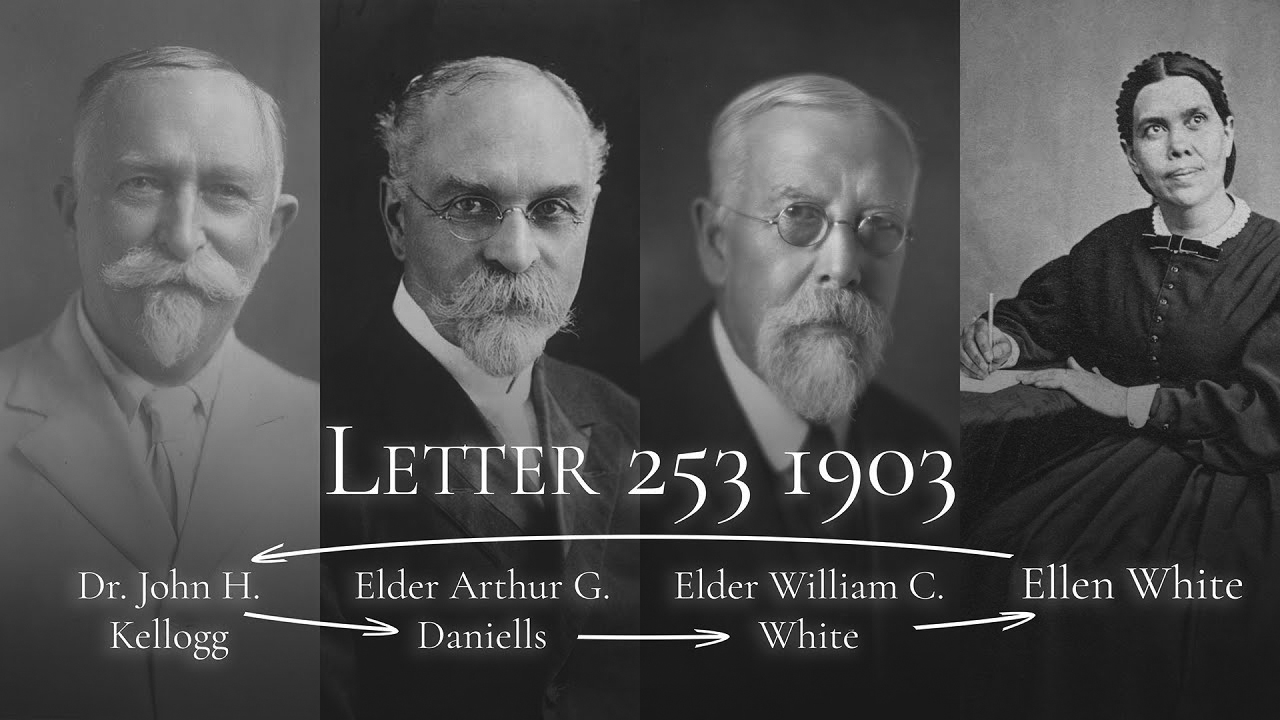
\includegraphics[width=1\linewidth]{images/correspondance.jpg}
    \caption*{Correspondence chain between A. G. Daniells, W. C. White, Ellen White and Dr. John H. Kellogg.}
    \label{fig:corespondance}
\end{figure}


\begin{figure}[h]
    \centering
    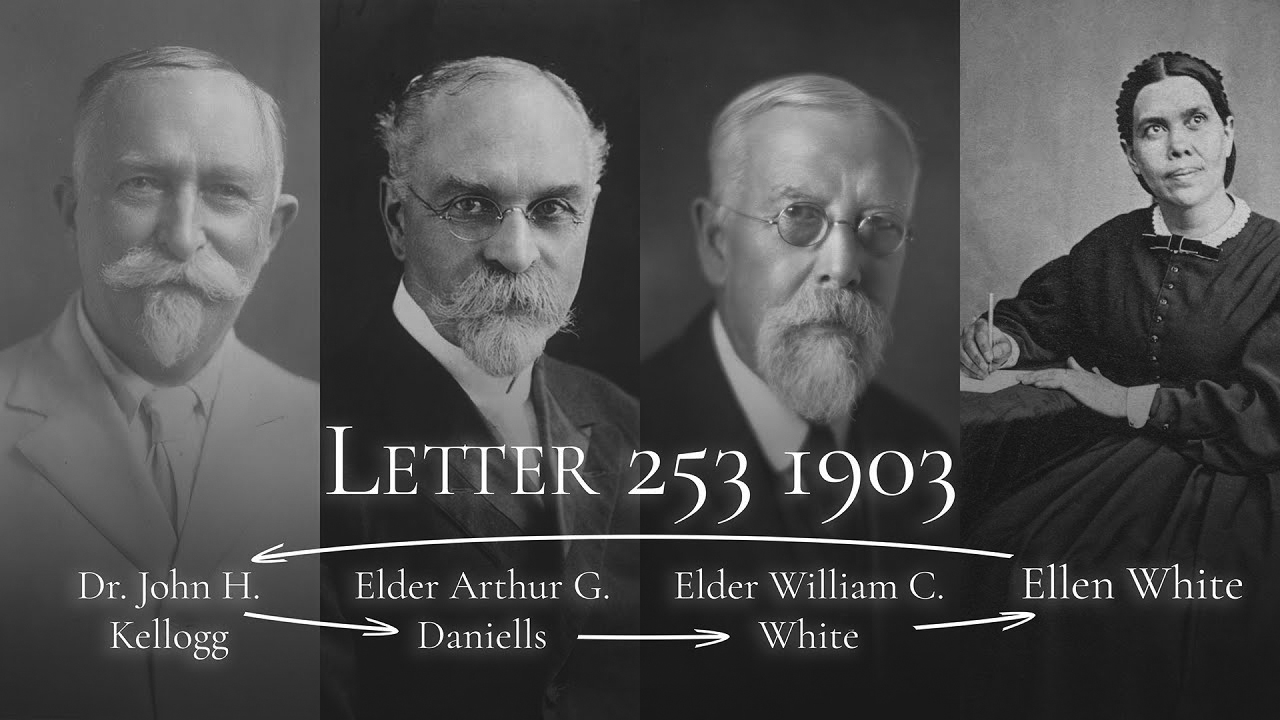
\includegraphics[width=1\linewidth]{images/correspondance.jpg}
    \caption*{Mfululizo wa mawasiliano kati ya A. G. Daniells, W. C. White, Ellen White na Dk. John H. Kellogg.}
    \label{fig:corespondance}
\end{figure}


Here is evidence that Sister White was familiar with Dr. Kellogg's intentions to revise “\textit{Living Temple}” and her familiarity with his belief in the Trinity doctrine. In William's words, she expressed herself quite emphatically regarding this matter. She deemed it an unprofitable undertaking. For this reason, it was necessary to issue a special Testimony soon. And there it was. This is how the \textit{Testimonies for the Church Containing Letters to Physicians and Ministers Instruction to Seventh-Day Adventists} was published in 1904, containing letters to the physicians and ministers connected to Kellogg's crisis.


Huu hapa ni ushahidi kwamba Dada White alikuwa anafahamu nia ya Dk. Kellogg ya kurekebisha “\textit{Hekalu Hai}” na kufahamiana kwake na imani yake katika Fundisho la Utatu. Kwa maneno ya William, yeye alijieleza kwa msisitizo kabisa kuhusiana na jambo hili. Aliona kuwa haina faida kufanya urekebisho. Kwa sababu hii, ilikuwa ni lazima kutoa Ushuhuda maalum hivi karibuni. Na vivyo ndivyo ushuhuda ulikuwepo. Hivi ndivyo \textit{Shuhuda za Kanisa zenye Barua kwa Madaktari na Maelekezo kwa Wahudumu kwa Waadventista Wasabato} ilichapishwa mwaka wa 1904, yenye barua kwa madaktari na wahudumu waliounganishwa na shida ya Kellogg.


By saying \others{\textbf{\underline{Mother and I} have just read your letter of \underline{October 29}}}, William testified that Sister White was fully aware of Kellogg's intentions and trinitarian belief. After she read Daniells’ letter, she wrote a direct reply to Dr. Kellogg. This letter is \textit{Lt253-1903}. It is a very prominent and eye opening letter because it clearly exposes how the prophet dealt with the Trinity doctrine. She elevated the doctrine on the \emcap{personality of God} constituted in the \emcap{Fundamental Principles}. There are striking similarities between this letter and the tenth chapter of the Special Testimonies, \textit{The Foundation of our Faith}.


Kwa kusema \others{\textbf{\underline{Mama pamoja nami} tumesoma sasa hivi barua yako ya \underline{Oktoba 29}}}, William alithibitisha kwamba Dada White alijua kikamilifu nia ya Kellogg na imani yake kuhusu utatu. Baada ya yeye kusoma Barua ya Daniells, aliandika jibu la moja kwa moja kwa Dk. Kellogg. Barua hii ni \textit{Lt253-1903}. Ni barua maarufu sana na ya kufungua macho kwa sababu inafichua wazi jinsi nabii alivyoshughulika na Fundisho la Utatu. Aliinua fundisho juu ya \emcap{Umbile la Mungu} ulio wekwa katika \emcap{Kanuni za Kimsingi}. Kuna kufanana wa kushangaza kati ya barua hii na ya sura ya kumi ya Shuhuda Maalum, \textit{Msingi wa Imani yetu}.


% Revision of the Living Temple

\begin{titledpoem}
    
    \stanza{
        In Kellogg’s book, a subtle snare \\
        Though well-disguised through crafty care \\
        From Bible truth would lead away \\
        And cause some precious souls to stray.
    }

    \stanza{
        And though much scripture there was used \\
        The early truth became confused \\
        This error served to twist the mind \\
        But in God’s Word the truth we find.
    }

    \stanza{
        God’s personality has form \\
        To Bible truth we must conform \\
        On this the Doctor wasn’t clear \\
        But early Advent truth is dear
    }
    
\end{titledpoem}


% Revision of the Living Temple

\begin{titledpoem}
    
    \stanza{
        In Kellogg’s book, a subtle snare \\
        Though well-disguised through crafty care \\
        From Bible truth would lead away \\
        And cause some precious souls to stray.
    }

    \stanza{
        And though much scripture there was used \\
        The early truth became confused \\
        This error served to twist the mind \\
        But in God’s Word the truth we find.
    }

    \stanza{
        God’s personality has form \\
        To Bible truth we must conform \\
        On this the Doctor wasn’t clear \\
        But early Advent truth is dear
    }
    
\end{titledpoem}
